%%%%%%%% ICML 2019 EXAMPLE LATEX SUBMISSION FILE %%%%%%%%%%%%%%%%%

\documentclass{article}

\usepackage[margin=1in]{geometry}
\usepackage{indentfirst}
% \usepackage{multibbl}

\usepackage[utf8]{inputenc} % allow utf-8 input
\usepackage[T1]{fontenc}    % use 8-bit T1 fonts
\usepackage{hyperref}       % hyperlinks
\usepackage{url}            % simple URL typesetting
\usepackage{booktabs}       % professional-quality tables
\usepackage{amsfonts}       % blackboard math symbols
\usepackage{nicefrac}       % compact symbols for 1/2, etc.
\usepackage{microtype}      % microtypography

\usepackage{bbm}
\usepackage{amsfonts}
\usepackage{amsmath,amsthm}           
\usepackage{mathtools}    
\usepackage{amsopn}
\usepackage{amssymb}
\usepackage{bm}
\usepackage{multirow}
\usepackage{graphicx}
\usepackage{float}
\usepackage{subfigure}
% \usepackage{subcaption}
\usepackage{adjustbox}
\usepackage{xcolor}
\usepackage[vlined,linesnumbered,ruled]{algorithm2e}
\usepackage{biblatex}


\newcommand{\avgR}{\wh{\cal{R}}}
\newcommand{\ips}{\wh{r}}
\newcommand{\whpi}{\wh{\pi}}
\newcommand{\whE}{\wh{\E}}
\newcommand{\whV}{\wh{V}}
\newcommand{\Reg}{\text{\rm Reg}}
\newcommand{\SA}{\text{\rm SA}}
\newcommand{\whReg}{\wh{\text{\rm Reg}}}
\newcommand{\flg}{\text{\rm flag}}
\newcommand{\one}{\boldsymbol{1}}
\newcommand{\var}{\Delta}
\newcommand{\p}{\prime}
\newcommand{\nb}{\nabla}
\newcommand{\epo}{\text{epoch}}

\DeclareMathOperator*{\arginf}{arginf}
\DeclareMathOperator*{\argsup}{argsup}
\DeclareMathOperator*{\range}{range}
\DeclareMathOperator*{\mydet}{det_{+}}
\DeclarePairedDelimiter\abs{\lvert}{\rvert}
\DeclarePairedDelimiter\bigabs{\big\lvert}{\big\rvert}
\DeclarePairedDelimiter\ceil{\lceil}{\rceil}
\DeclarePairedDelimiter\floor{\lfloor}{\rfloor}
\DeclarePairedDelimiter\bigceil{\big\lceil}{\big\rceil}
\DeclarePairedDelimiter\bigfloor{\big\lfloor}{\big\rfloor}

\newcommand{\field}[1]{\mathbb{#1}}
\newcommand{\fY}{\field{Y}}
\newcommand{\fX}{\field{X}}
\newcommand{\fH}{\field{H}}
\newcommand{\fR}{\field{R}}
\newcommand{\fN}{\field{N}}
\newcommand{\E}{\field{E}}

\newcommand{\theset}[2]{ \left\{ {#1} \,:\, {#2} \right\} }
\newcommand{\inner}[1]{ \left\langle {#1} \right\rangle }
\newcommand{\Ind}[1]{ \field{I}_{\{{#1}\}} }
\newcommand{\eye}[1]{ \boldsymbol{I}_{#1} }
\newcommand{\norm}[1]{\left\|{#1}\right\|}
%\newcommand{\trace}[1]{\text{tr}\left({#1}\right)}
\newcommand{\trace}[1]{\textsc{tr}({#1})}
\newcommand{\diag}[1]{\mathrm{diag}\!\left\{{#1}\right\}}
\newcommand{\UB}{\text{UB}}
\newcommand{\defeq}{\stackrel{\rm def}{=}}
\newcommand{\sgn}{\mbox{\sc sgn}}
\newcommand{\scI}{\mathcal{I}}
\newcommand{\scO}{\mathcal{O}}
\newcommand{\scN}{\mathcal{N}}
\newcommand{\order}{\ensuremath{\mathcal{O}}}
\newcommand{\otil}{\ensuremath{\widetilde{\mathcal{O}}}}
% \newcommand{\Pr}{\ensuremath{\mathrm{Pr}}}

\newcommand{\dt}{\displaystyle}
\renewcommand{\ss}{\subseteq}
\newcommand{\wh}{\widehat}
\newcommand{\wt}{\widetilde}
\newcommand{\ve}{\varepsilon}
\newcommand{\hlambda}{\wh{\lambda}}
\newcommand{\yhat}{\wh{y}}

\newcommand{\hDelta}{\wh{\Delta}}
\newcommand{\hdelta}{\wh{\delta}}
\newcommand{\spin}{\{-1,+1\}}
\newcommand\numberthis{\addtocounter{equation}{1}\tag{\theequation}}

\newcommand{\mc}[1]{\mathcal{#1}}
\newcommand{\mb}[1]{\mathbb{#1}}
\newcommand{\mr}[1]{\mathrm{#1}}

%%%%%%%%%%%%%%%%%%%%%%%%

\newtheorem{assumption}{Assumption}
\newtheorem{theorem}{Theorem}
\newtheorem{lemma}{Lemma}
\newtheorem{corollary}[theorem]{Corollary}
\newtheorem{proposition}{Proposition}
\newtheorem{definition}{Definition}
\newtheorem{remark}{Remark}
\DeclareMathOperator{\val}{val}
\DeclareMathOperator{\spa}{sp}
\DeclareMathOperator{\solve}{solve}
\allowdisplaybreaks

% Packages hyperref and algorithmic misbehave sometimes.  We can fix
% this with the following command.
%\newcommand{\theHalgorithm}{\arabic{algorithm}}

\DeclareMathOperator*{\argmin}{\arg\!\min}
\DeclareMathOperator*{\argmax}{\arg\!\max}
% \setlength\parindent{10pt}

\newcommand{\compilefullversion}{true}%SHOW short version
\ifthenelse{\equal{\compilefullversion}{false}}{%
    \newcommand{\OnlyInFull}[1]{}
    \newcommand{\OnlyInShort}[1]{#1}
}{%
    \newcommand{\OnlyInFull}[1]{#1}%
    \newcommand{\OnlyInShort}[1]{}%
}%

% Macro for comments:
% \newcommand{\compilehidecomments}{false}%HIDE comments

% \ifthenelse{\equal{\compilehidecomments}{true}}{%
%     \newcommand{\wei}[1]{}
%     \newcommand{\haoyu}[1]{}
%     \newcommand{\kai}[1]{}
% }{
%     \newcommand{\wei}[1]{{\color{blue!50!black}  [\text{Wei:} #1]}}
%     \newcommand{\haoyu}[1]{{\color{brown!60!black} [\text{Haoyu:} #1]}}
%     \newcommand{\kai}[1]{{\color{purple} [\text{Kai:} #1]}}
% }


\allowdisplaybreaks

\title{Offline reinforcement learning with delay rewards}
\author{
xxx\\
Nanjing University\\
\texttt{xxx}
\and
xxx\\
Kuaishou Corp.\\
\texttt{xxx}
}
\date{}

\addbibresource{reference.bib}
% \newbibliography{main}
% \newbibliography{appendix}

\begin{document}
\maketitle

\begin{abstract}  
blablabla
\end{abstract}

\section{Introduction}

This is introduction part.




\section{Related work}


\section{Preliminaries}\label{sec:prel}

\subsection{Offline reinforcement learning}


\section{Method}{\label{sec: method}}

In this section, we present a general framework for addressing delay rewards or sparse rewards problems in offline setting. From a global perspective, the framework consists of two-stage learning tasks, in the first stage we perform reward modification strategy on the offline datasets, and then learn the offline policy from the modified datasets in the latter stage.

\subsection{Reward modification} 

Our starting point is to find an appropriate conversion function of the original delayed rewards, such modification restores a dense reward as much as possible so that helps the offline policy learning phase afterwards. Such conversion only occurs at the offline data level, and any offline policy learning algorithm can be seamlessly combined with it in the subsequent strategy learning phase.

Next, we will introduce 3 kinds of reward conversion strategies:

\begin{enumerate}
    \item \textbf{Reward Decomposition.} Works in this area \cite{arjona-medinaRUDDERReturnDecomposition2019} consider establishing a decomposition strategy to convert the original delay or sparse rewards into dense rewards under constraints. We can train a parameterized reward network $f_{\theta}(s, a)$ from the original delay rewards (sparse) data obeying that for a trajectory $\tau = \left(s_0, a_0, r_0, \cdots,  s_T, a_T, r_T\right)$ sampled from offline datasets $\mathcal D$, the decomposition operation keeps the decomposed reward $r_t' = f_{\theta}(s_t, a_t)$ and the original reward $r$ to be consistent on the trajectory level, that is: $\sum_{t = 0}^T r_t = \sum_{t = 0}^T r_t'$.
    
    \item \textbf{Reward Shaping.} Reward shaping is well studied as it maintains the invariance of policy before and after the reward transformations. We follow the prior work \cite{ngPolicyInvarianceReward1999} by adding an extra bounded real-valued shaping function $F: \mathcal S \times \mathcal A \times S \rightarrow \mathbb R$ to the raw reward function $R$, in practice, we parameterize this shaping reward function by differentiable neural network and train it with Policy Gradient methods \cite{Peters:2010}.

    \item \textbf{Reward Smoothing.} Delay rewards deviate greatly from the immediate reward in scale and space, smoothing is the strategy that attemps to re-distribute the single step delayed reward $r_t^{delay}$ to multi-step immediate rewards $r_{t - k: t}$ satisfying the constraints that it keeps the consistency of the reward sum in the interval $[t - k: t]$: $\sum_{i = t-k}^t r_t = r_t^{delay}$. 
	Specifically, we consider the following smoothing transformations:
	\begin{enumerate}
		\item \textbf{Minmax strategy}.

		\item \textbf{Average strategy}.

		\item \textbf{Ensemble strategy}.

	\end{enumerate}
    
\end{enumerate}

\subsection{Offline policy learning}

In offline scenarios, trial-and-error and exploration of the environment becomes impossible, and delaying the reward signal in most cases introduces the problem of reward sparsity, which makes the conventional optimization algorithm that maximizing the expected rewards from offline data no longer applicable. Our goal is to find the optimal policy $\pi^{*} = \arg \max_{\pi} \mathbb E_{\tau \in \mathcal D} \left[ R_{\tau} \right]$ that maximizes the cumulative reward from this offline datasets with delayed rewards.




\section{Experiments}

In this section, we conducted corresponding experiments in the D4RL public datasets and the real-world recommendation system scenarios. Our primary points of comparison are reward modification strategies include: scale, return min-max, average, ensemble. Furthermore, these strategies can be combined with any offline RL algorithms without extra efforts, model-free offline RL algorithms BC, CQL and model-based algorithm MOPO are included depend on the environment as follows:

\begin{itemize}
    \item Behaviour Cloning(BC). BC uses supervised learning for policy learning, and the learning process does not depend on the rewards. Therefore, delaying the rewards has no effect on its policy learning process. In this part, we directly quote the results published in the D4RL paper.
    
    \item Conservative Q-Learning(CQL). CQL is a type of model-free algorithm. It learns a Q-value function directly from the data, thereby avoiding action out of distribution(OOD) caused by offline reinforcement learning.
    
    \item Model-based Offline Policy Optimization(MOPO). MOPO is a model-based algorithm. It first learns multiple supervised learning models (including state transition and reward function) from offline data, and the strategy interacts with the learned model. The reward adds an additional transition to the joint model. Deterministic estimation, as an empirical reward Lower Bound, has verified its effectiveness in theory and experiment.
    
\end{itemize}

we verify the effectiveness of aforementioned methods in solving the delayed rewards problems. Experiments conducted both on simuated offline datasets (OpenAI Gym) and customized real-world datasets. All tasks involves delayed rewards and high-dimensional observation spaces, xxx.

\subsection{Evaluation on D4RL public datasets}

In this section, we compare to BC, CQL, and MOPO on three continuous control tasks from the D4RL bechmark. As the original datasets We first construct the delay rewards datasets from the original none-delayed rewards datasets on 4 levels setting:

\begin{enumerate}
    \item Random: 1 million timesteps generated by a “random” policy.
    \item Medium: 1 million timesteps generated by a “medium” policy that achieves approximately one-third the score of an expert policy.
    \item Medium-Replay: the replay buffer of an agent trained to the performance of a medium policy (approximately 25k-400k timesteps in our environments).
    \item Medium-Expert: 1 million timesteps generated by the medium policy concatenated with 1 million timesteps generated by an expert policy.
\end{enumerate}

\textbf{Datasets construction.} In order to make a public comparison with other offline algorithms, we delay the dense reward based on the D4RL gym datasets. Specifically, we perform constant delay setting: we set a hyper-parameter $K$ as the delay interval which controls the sparsity of the delayed rewards. We set the delayed reward at equal intervals with $K$ as the un-discounted cumulative rewards of corresponding interval, the missing reward filled with 0, formally:

For a trajectory $\tau$ with length $T$, we set the delayed reward of time step $t$ as $r_t^{delay}$, where:

$$
\begin{aligned}
r_t^{delay} = \begin{cases}
0, \text{if} \ t \mod K \neq 0; \\
\sum_{i = t - K + 1}^t r_t, \text{otherwise}.
\end{cases}
\end{aligned}
$$

Such construction strategy introduce sparsity to delay rewards, meanwhile, it keeps the rule that for any trajectory in the original datasets, the un-discounted cumulative rewards keep constant before and after the operation, mathematically, we have:

$$
\sum_{t = 1}^{T} r_t = \sum_{t = 1}^{T} r_t^{delay}
$$

To facilitate intuitive and clear comparison of the delay reward:
\begin{figure}[H]
    \centering
    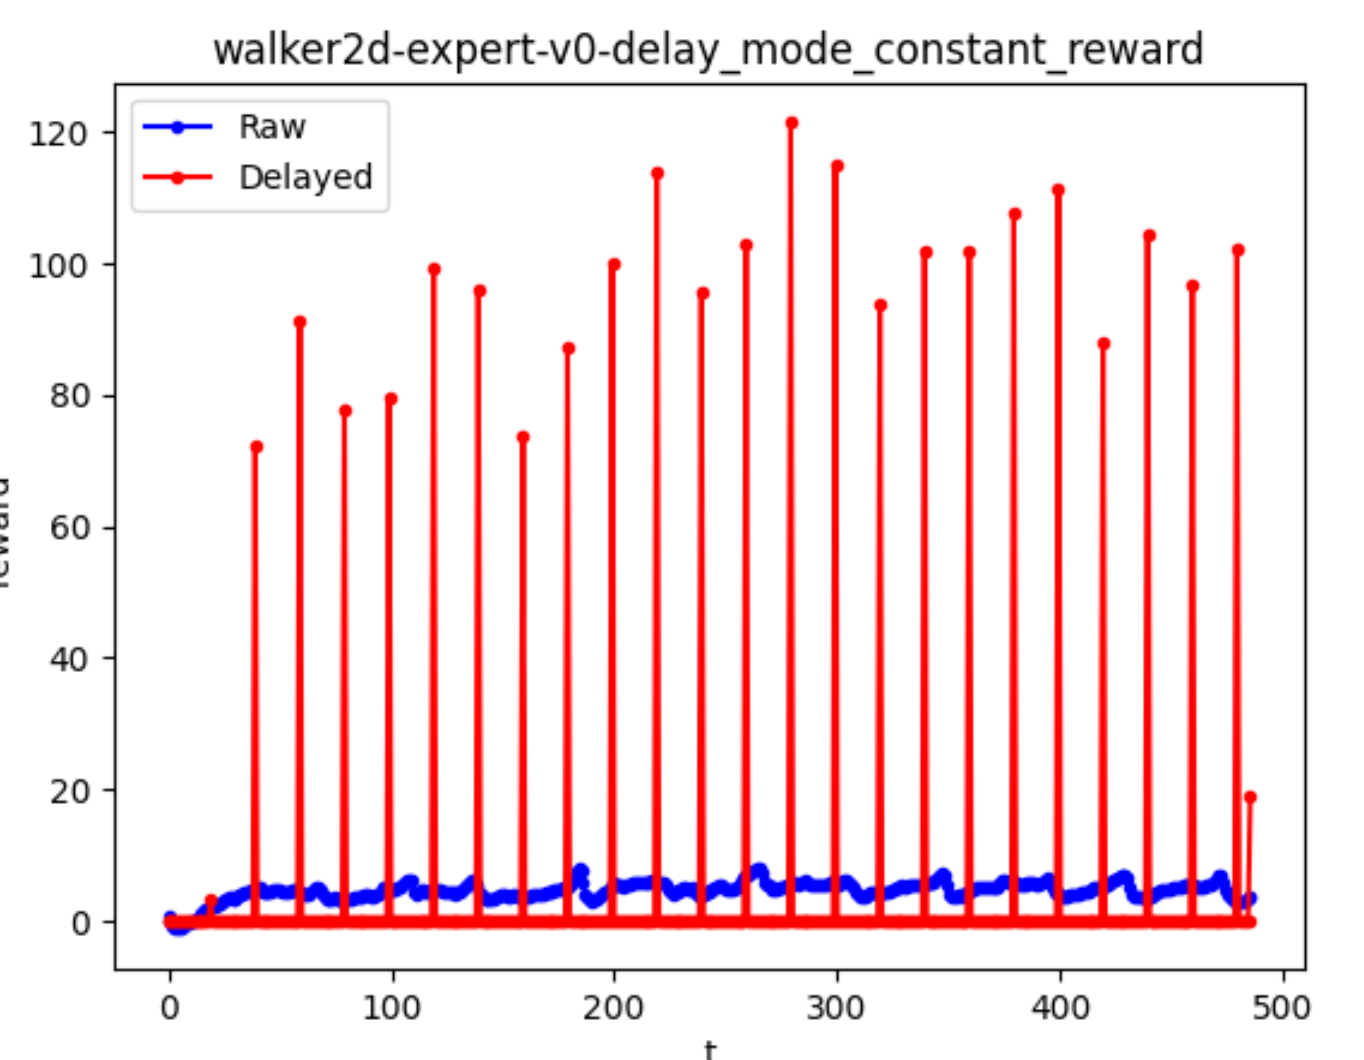
\includegraphics[width=0.95\textwidth]{assets/image.png}
    \caption{Delayed rewards xxx}
    \label{fig:fig1}
\end{figure}


We compare to BC, CQL, and MOPO. BC numbers are reported from the original D4RL paper, CQL and MOPO results are run by us. Our results are shown in Table 1. MOPO(average) achieves the highest scores in 11/12 of the tasks.


\begin{table*}[h]
\centering
\begin{tabular}{lll|cc|ccc}
\toprule
& & & & & \multicolumn{3}{c}{\bf MOPO} \\
\multicolumn{1}{l}{\bf Dataset} & \multicolumn{1}{c}{\bf Environment} & \multicolumn{1}{c|}{\bf Delay} & \multicolumn{1}{c}{\bf BC} & \multicolumn{1}{c|}{\bf CQL} & \multicolumn{1}{c}{\bf{Normal}} & \multicolumn{1}{c}{\bf +Average} & \multicolumn{1}{c}{\bf +Ensemble}\\
\midrule
Random        & HalfCheetah &  20 & $2.1$ &  -  &  $0.1$ &  $\bf{25.3 \pm 1.5 }$ \\
Random        & Hopper      &  20 & $1.6$ &  -  &  $3.1$ &  $\bf{9.1 \pm 1.5 }$ \\
Random        & Walker2d    &  20 & $9.8$ &  -  &  $0.1$ &  $\bf{12.6 \pm 6.1 }$ \\
\midrule
Medium        & HalfCheetah &  20 & $36.1$ &  - &  $-0.8$ &  $\bf{48.3 \pm 2.4}$ \\
Medium        & Hopper      &  20 & $29$ & - & $5.1$ &  $19.0 \pm 8.1$ \\
Medium        & Walker2d    &  20 & $6.6$ & - & $4.5$ &  $\bf{72.3 \pm 0.9}$ \\
\midrule
Medium-Replay & HalfCheetah &  20 & $38.4$ & - & $1.9$ &  $54.5 \pm 3.2$ \\
Medium-Replay & Hopper      &  20 & $11.8$ & - & $1.9$ &  $89.8 \pm 5.7$ \\
Medium-Replay & Walker2d    &  20 & $11.3$ & - & $0.9$ &  $\bf{59.1 \pm 3.7}$ \\
\midrule
Medium-Expert & HalfCheetah &  20 & $35.8$ & - & $2.1$ &  $\bf{73.6 \pm 8.3}$ \\
Medium-Expert & Hopper      &  20 & $111.9$ & - & $9.4$ &  $\bf{22.1 \pm 3.2}$ \\
Medium-Expert & Walker2d    &  20 & $6.4$  & - & $6.8$ & $\bf{99.0 \pm 3.7}$\\
\bottomrule
\end{tabular}
\caption{
Results for D4RL datasets\protect\footnotemark.
We report the mean and variance for three seeds.
MOPO+Average outperforms conventional RL algorithms on almost all tasks.}
\label{tbl:mujoco_results}
\end{table*}

\subsection{Evaluation on recommender system simulated datasets}
In order to verify the effectiveness of the reward modification strategy proposed in the article, we added a simulation environment in a real-world scenario for verification.





\section{Conclusions}
In this paper, we propose a xxx.  



% \begin{ack}
% Use unnumbered first level headings for the acknowledgments. All acknowledgments
% go at the end of the paper before the list of references. Moreover, you are required to declare 
% funding (financial activities supporting the submitted work) and competing interests (related financial activities outside the submitted work). 
% More information about this disclosure can be found at: \url{https://neurips.cc/Conferences/2020/PaperInformation/FundingDisclosure}.


% Do {\bf not} include this section in the anonymized submission, only in the final paper. You can use the \texttt{ack} environment provided in the style file to autmoatically hide this section in the anonymized submission.
% \end{ack}

\newpage
% \bibliographystyle{abbrvnat}
% \bibliographystyle{plainnat}
% \bibliography{reference} 

\printbibliography

% \bibliographystyle{main}{plain}
% \bibliography{main}{reference}{reference}
   

\newpage
\appendix
% \begin{refsection}
\section*{Appendix}
\addcontentsline{toc}{section}{Appendices}
% \renewcommand{\thesubsection}{\Alph{subsection}}

\section{Reward Modification Implementation Details}
\label{appendix: rm_imp_details}
XXXX

\section{Experiment Details}
\label{appendix: exp_details}
Our implementation is based on the OfflineRL library released by NeoRL team.
For all experiments, we used default hyperparameter settings and minimal 
modifications to public implementations wherever possible, with different 
training iterations or gradient steps depending on the algorithm. We ran our 
experiments using single 1080 GPU machines.

\subsection{D4RL benchmark}\label{appendix: exp_d4rl_details}
XXX

\subsection{Custom simulated environment}\label{appendix: exp_custom_detials}
We build our simulated environment on the RecSim framework for its flexibility and scalability, RecSim is published by 
google research team to build a configurable platform for building simulated environments 
for recommender systems (RSs) that naturally supports sequential interaction with users.

Datasets are collected by pretraining an agent in Soft Actor-Critic way from scratch and collecting 1000 trajectories at 4 different levels:

\begin{itemize}
    \item Random: 
    \item Low: 
    \item Medium: 
    \item Expert:
\end{itemize}


% \printbibliography[heading=subbibliography]
% \end{refsection}

% \bibliographystyle{appendix}{plain}
% \bibliography{appendix}{reference}{reference}




\end{document}